\documentclass[10pt,a4paper,headinclude,twoside, plainheadsepline, open=right, numbers=noenddot, twocolumn]{article}
%
% ------
% Maketitle metadata
\title{\vspace{-5mm}%
	\fontsize{20pt}{10pt}\selectfont
	\textbf{Messung der Hydratation durch tragbare Photoplethysmographie-Sensoren}
	}	
\vspace{-5mm}\date{}
\author{
	\large
       \begin{minipage}[t]{0.33\linewidth}
         \begin{center}
           	\textsc{Olga Litau}\\[2mm]
                 \normalsize	Matr.Nr: 3156218\\
                 \normalsize
                 \href{mailto:olga1.litau@st.oth-regensburg.de}
                 {olga1.litau@st.oth-regensburg.de}      
         \end{center}
       \end{minipage}        
     }
%
%\addto\captionsgerman{\renewcommand{\figurename}{Fig.}}
%
%%%%%%%%%%%%%%%%%%%%%%%%%%%%%%%%%%%%%%%%%%%%%%%%%%%%%%%%%%%
%
% Literaturverzeichnis
%
% Hier eine von zwei Varianten auswaehlen:
% Nummern oder Buchstaben fuer Referenzen
%\usepackage[backend=biber, style=alphabetic, sorting=nyt]{biblatex}
\usepackage[backend=biber, style=numeric-comp, sorting=none]{biblatex}
\usepackage{booktabs}
%
% Hier werden die Referenzen in einer separaten Datei gespeichert
\addbibresource{termPaper.bib}
%
% WICHTIG: Hier wird nicht BibTeX sondern BibLateX verwendet!!
% Deshalb nicht mit bibtex uebersetzen, sondern mit biber
% Das kann man in jedem Tool wie TexMaker oder TexShop als Option einstellen
%

% Spezielle Einstellungen, insbesondere fuer das Literaturverzeichnis,
% aber auch Packages wie amsmath, Groessenanpassungen etc.
% Allgemeines
%\usepackage[automark]{scrpage2} % Kopf- und Fusszeilen
\usepackage{amsmath} % Mathematik
\usepackage{amsfonts}
\usepackage{amssymb}
\usepackage[utf8]{inputenc} % UTF8-Kodierung fuer Umlaute usw
\usepackage{hyperref} % Internetseiten
\usepackage{multirow} % Tabellen-Zellen ueber mehrere Zeilen
\usepackage{multicol} % mehre Spalten auf eine Seite
\usepackage{tabularx} % Fuer Tabellen mit vorgegeben Groessen
\usepackage[ngerman]{babel}
\usepackage{graphicx} % Bilder
\usepackage{epstopdf} % enable eps graphics
\usepackage{color} % Farben
\usepackage{subfig} % mehrere Abbildungen nebeneinander/uebereinander
% Quellcode
\usepackage{listings} % fuer Formatierung in Quelltexten
\usepackage[font=small,labelfont=bf,figurename=Abb.,tablename=Tab.]{caption}
\usepackage{capt-of}
%%%%%%%%%%%%%%%%%%%%%%%%%%%%%%%%%%%%%%%%%%%%%%%%%%%%%%%%%%%
% ------
% Fonts and typesetting settings
\usepackage[sc]{mathpazo}
\usepackage[T1]{fontenc}
\usepackage{microtype}
% ------
% Page layout
\usepackage[hmarginratio=1:1,top=32mm,columnsep=20pt]{geometry}
\usepackage[font=it]{caption}
\usepackage{paralist}

% ------
% Abstract
\usepackage{abstract}
	\renewcommand{\abstractnamefont}{\normalfont\bfseries}
	\renewcommand{\abstracttextfont}{\normalfont\small\itshape}
%
%
% ------
% Titling (section/subsection)
\usepackage{titlesec}
\titleformat{\section}[block]{\large\scshape\centering}{\thesection.}{1em}{}
%
%%%%%%%%%%%%%%%%%%%%%%%%%%%%%%%%%%%%%%%%%%%%%%%%%%%%%%%%%%%
%
% Einstellungen zum Literaturverzeichnis
%
% Anpassen bei "alphabetic"
\ExecuteBibliographyOptions{%
     maxbibnames=99,   % Alle Autoren (kein et al.)
     maxcitenames=1,   % Kuerzel nur aus 1. Autor im Text
     maxalphanames=1,  % nur 1. Autor in der Abkuerzung
     backref=false,    % keine Ruueckverweise auf Zitatseiten
     firstinits=true,  % Vornamen abkuerzen
     isbn=false,       % ISBN ausblenden
     doi=false,        % DOI ausblenden
   }
\renewcommand*{\labelalphaothers}{} % alpha label ohne +
%
\renewbibmacro*{volume+number+eid}{%
     \setunit{\space}\printfield{volume}%
     \iffieldundef{number}{}{%
      \printtext[parens]{\printfield{number}}}%
     \setunit{\addcomma\space}\printfield{eid}}
%
% no word 'pages' for articles in the bibliography (print as is)
\DeclareFieldFormat[article, inproceedings, incollection, unpublished]{pages}{#1} 
% no quotes for article titles (print as is)
\DeclareFieldFormat[article, inproceedings, incollection, online, unpublished]{title}{#1} 
%
\renewbibmacro*{date}{\printdate}
\renewbibmacro*{issue+date}{\usebibmacro{issue}}
\renewbibmacro*{publisher+location+date}{\printlist{publisher}}
%
   \setcounter{biburlnumpenalty}{9000}
   \setcounter{biburlucpenalty}{9000}
   \setcounter{biburllcpenalty}{9999}
%
% "In:" removed for articles; issue/date macros added after note+pages macro
\DeclareBibliographyDriver{article}{%
  \usebibmacro{bibindex}%
  \usebibmacro{begentry}%
  \usebibmacro{author/translator+others}%
  \setunit{\labelnamepunct}\newblock%
  \usebibmacro{title}%
  \newunit%
  \printlist{language}%
  \newunit\newblock%
  \usebibmacro{byauthor}%
  \newunit\newblock%
  \usebibmacro{bytranslator+others}%
  \newunit\newblock%
  \printfield{version}%
  \newunit\newblock%
  \usebibmacro{journal+issuetitle}%
  \newunit%
  \usebibmacro{byeditor+others}%
  \newunit%
  \usebibmacro{note+pages}%
  \setunit{\addcomma\addspace}%
  \usebibmacro{date}%
  \usebibmacro{finentry}}
%
%
\DeclareBibliographyDriver{inproceedings}{%
    \usebibmacro{begentry}%
    \printnames{author}%
    \setunit{\labelnamepunct}\newblock%
    \printfield{title}%
    \setunit{\labelnamepunct}%
	\usebibmacro{in:}%    
    \newblock%
    \ifnameundef{editor}%
    {%
    		\setunit{\adddot\space}%
    		\newunit%
    }%
    {%
     	\setunit{\addspace}%
     	\printnames[byeditor]{editor}%
     	\clearname{editor}%
     	\setunit{\space}%
     	\printtext[parens]{Hrsg.}%
     	\setunit{\addcolon\space}%
     	\newunit%
     }%
	\printfield{booktitle}%
	\setunit{\addcomma\space}%
	\printfield{pages}%
	\setunit{\addcomma\space}%
    \usebibmacro{date}%
    \usebibmacro{finentry}
}

\DeclareBibliographyDriver{book}{%
  \usebibmacro{bibindex}%
  \usebibmacro{begentry}%
  \usebibmacro{author/editor+others/translator+others}%
  \setunit{\labelnamepunct}\newblock
  \usebibmacro{maintitle+title}%
  \newunit
  \printlist{language}%
  \newunit\newblock
  \usebibmacro{byauthor}%
  \newunit\newblock
  \usebibmacro{byeditor+others}%
  \newunit\newblock
  \printfield{edition}%
  \newunit
  \iffieldundef{maintitle}
    {\printfield{volume}%
     \printfield{part}}
    {}%
  \newunit
  \printfield{volumes}%
  \newunit\newblock
  \usebibmacro{series+number}%
  \newunit\newblock
  \printfield{note}%
  \newunit\newblock
  \usebibmacro{publisher+location+date}%
  \newunit\newblock
  \usebibmacro{chapter+pages}%
  \newunit
  \printfield{pagetotal}%
  \newunit\newblock
  \usebibmacro{doi+eprint+url}%
  \newunit\newblock
  \usebibmacro{addendum+pubstate}%
  \setunit{\bibpagerefpunct}\newblock
  \usebibmacro{pageref}%
  \setunit{\addcomma\space}
  \usebibmacro{date}
  \usebibmacro{finentry}}
%  
%
 \DeclareBibliographyDriver{online}{%
   \usebibmacro{bibindex}%
   \usebibmacro{begentry}%
   \ifnameundef{author}
    {\printtext{Autor unbekannt}}
    {
		\usebibmacro{author/editor+others/translator+others}%    
    }%
   \setunit{\labelnamepunct}\newblock
   \usebibmacro{title}%
   \newunitpunct
   \usebibmacro{url+urldate}%
   %\usebibmacro{addendum+pubstate}%
   \usebibmacro{finentry}}  
%%%%%%%%%%%%%%%%%%%%%%%%%%%%%%%%%%%%%%%%%%%%%%%%%%%%%%%%%%%

% Eigene Befehle %%%%%%%%%%%%%%%%%%%%%%%%%%%%%%%%%%%%%%%%%%%%%%%%%
% Matrix
\newcommand{\mat}[1]{
      {\textbf{#1}}
}
\newcommand{\todo}[1]{
      {\colorbox{red}{ TODO: #1 }}
}
\newcommand{\todotext}[1]{
      {\color{red} TODO: #1} \normalfont
}
\newcommand{\info}[1]{
      {\colorbox{blue}{ (INFO: #1)}}
}
\newcommand{\code}[1]{
      {\ttfamily{#1}}
}

%%%%%%%%%%%%%%%%%%%%%%%%%%%%%%%%%%%%%%%%%%%%%%%%%%%%%%
% Groessenanpassungen
%
\setlength{\unitlength}{1cm}
\setlength{\oddsidemargin}{0.3cm}
\setlength{\evensidemargin}{0.3cm}
\setlength{\textwidth}{15.5cm}
\setlength{\topmargin}{-1.2cm}
\setlength{\textheight}{23cm}
\columnsep 0.5cm

%
% ------
% Header/footer
\usepackage{fancyhdr}
	\pagestyle{fancy}
	\fancyfoot[C]{Wissenschaftliches Seminar WS 2018/19 $\cdot$
          $\cdot$ Prof.~Dr.~Doering}
%
	\fancyhead[RE]{Olga Litau}
	\fancyhead[LO]{Messung der Hydratation durch tragbare Photoplethysmographie
Sensoren}	
	\fancyhead[RO,LE]{\thepage}
%
\begin{document}
\pagenumbering{arabic} % ab jetzt arabische Nummerierung
\twocolumn[
%%%%%%%%%%%%%%%%%%%%%%%%%%%%%%%%%%%%%%%%%%%%%%%%%%%%%%%%%%%%%%%%%%%%%
\maketitle
\tableofcontents % Inhaltsverzeichnis
\vspace{2cm}
\begin{abstract}
\noindent 
Diese Arbeit behandelt die Verwendung von tragbaren Photoplethysmographie (PPG) Sensoren zur Untersuchung von Veränderungen des Körperwassers. 
Zunächst werden etablierte Methoden wie die klinische Anamnese und Laboruntersuchungen vorgestellt.
Es wird weiterhin erläutert wie PPG-Sensoren zur physiologischen Messung genutzt werden und wie ein solches Signal verarbeitet werden muss, um daraus den Hydratationszustand einer Person abzuleiten. 
Abschließend werden die PPG-Sensoren im Vergleich mit den etablierten Methoden bewertet.
PPG-Sensoren sind tragbar, nicht invasiv und können kontinuierlich zur Überwachung des Hydratationszustandes eingesetzt werden.
Jedoch hängt die Genauigkeit und Zuverlässigkeit der Messergebnisse von der Qualität der verwendeten Algorithmen zur Verarbeitung des PPG-Signals und der Merkmalsextraktion ab.

\end{abstract}
\vspace{0.2cm}
]


\section{Einleitung}
\label{einleitung}
Dehydratation bezeichnet eine übermäßige Abnahme des Körperwassers, die eine normale tägliche Schwankung überschreitet. 
Mit 50-70\% der Gesamtkörpermasse ist Wasser der chemische Hauptbestandteil des menschlichen Körpers.
Für einen durchschnittlichen jungen Mann mit 70kg Körpergewicht bedeutet das ein Gesamtkörperwasser von 42l \cite{sawka2015hypohydration}.
5-10\% des Gesamtkörperwassers werden täglich umgesetzt \cite{raman2004american}.
Ein Körperwasserdefizit entsteht wenn die Flüssigkeitsaufnahme durch Getränke und Lebensmittel geringer ist als die Ausscheidung durch Urin, Schweiß, Kot und Verdunstung aus den Atemwegen und der Haut \cite{garret2018engineering}.
Der Begriff "Dehydratation" wird häufig als Synonym für hypertone Dehydratation verwendet.
Unter hypertoner Dehydratation versteht man einen Verlust von Wasser ohne entsprechenden Salzverlust. 
Verursacht werden kann eine hypertone Dehydratation durch unzureichende Flüssigkeitsaufnahme, Schwitzen oder Erbrechen.
Diese Form der Dehydratation ist zu unterscheiden von isotoner Dehydratation und hypotoner Dehydratation.
Isotone Dehydratation kennzeichnet einen Verlust von Wasser und Salz-Ionen im gleichen Verhältnis.
Eine isotone Dehydratation tritt beispielsweise als Folge von Durchfall auf.
Hypotone Dehydratation entsteht, wenn im Verhältnis zum Wasserverlust zu viel Salz ausgeschieden wird.
Bei der Verwendung eines Diuretikums, das die vermehrte Ausschwemmung von Urin aus dem menschlichen Körper bewirkt, kann eine hypotone Dehydratation verursacht werden. 
Bei einer Messung ist es von Vorteil zwischen den Arten der Dehydratation differenzieren zu können, um eine effektive Behandlung zu ermöglichen \cite{garret2018engineering}.

Die etablierten Methoden zur Messung der Dehydratation reichen von der klinischen Anamnese zu unterschiedlichen Untersuchungen im Labor.
Kapitel \ref{methoden zur messung der hydratation} wird einen Überblick über die verschiedenen Methoden geben. 

Neben den etablierten Methoden entwickeln sich verschiedene neue Ansätze zur Messung der Hydratation.
In dieser Arbeit wird die Messung durch tragbare Photoplethysmographie (PPG) Sensoren vorgestellt und bewertet.
Kapitel \ref{tragbare photoplethysmographie sensoren} richtet den Fokus auf tragbare PPG-Sensoren und erläutert sowohl die Verwendung von Photopletysmographie zur physiologischen Messung als auch die Verarbeitung eines PPG-Signals, um daraus Informationen über den Hydratationszustand einer Person zu entnehmen.
Abschließend erfolgt in Kapitel \ref{schlussbetrachtung und ausblick} eine Schlussbetrachtung der PPG-Sensoren im Vergleich zu etablierten Methoden sowie ein Ausblick. 



\section{Etablierte Methoden zur Messung der Hydratation}
\label{methoden zur messung der hydratation}

\begin{table*}[ht]
%\begingroup
\centering
\begin{tabular*}{10cm}{p{4.5cm}p{4.5cm}}
\toprule
\multicolumn{2}{c}{\textbf{Etablierte Methoden}} \\
 \midrule
Klinische Anamnese & Laboruntersuchungen  \\
\cmidrule(r){1-1}\cmidrule(l){2-2}
Durst & Blutanalyse \\
Hautturgor & Urinanalyse  \\
Blutdruck & Messung des Gewichts  \\
Herzfrequenz & Bioimpedanzanalyse  \\
\bottomrule
\end{tabular*}
\caption{Überblick über die rtablierten Methoden zur Messung der Hydratation.}
\label{methodenübersicht}
\end{table*}
%\endgroup


Um eine Grundlage für die Bewertung von PPG-Sensoren zu schaffen, werden in diesem Kapitel die verbreiteten Methoden zur Messung der Hydratation (vergleiche Tab.~\ref{methodenübersicht}) vorgestellt.
Von einer Dehydratation spricht man bei einem Wasserverlust von 3\% des Gesamtkörperwassers oder etwa 2\% des Körpergewichts für eine durchschnittliche Person.
Jedoch können bestimmte Risikogruppen wie z.B. ältere Erwachsene bereits Symptome mit weniger ausgeprägten Änderungen der Dehydratation aufweisen \cite{garret2018engineering}.

\subsection{Klinische Anamnese}
\label{klinische anamnese}

Klinische Anamnese wird häufig zur Beurteilung des Hydratationszustandes verwendet.
Dabei werden Symptome betrachtet, die vom Patienten wahrgenommen oder vom praktizierenden Arzt erkannt werden.

Die einfachste Maßnahme besteht darin, den Durst einer Person zu beurteilen, indem man Methoden wie eine visuelle Analogskala oder eine kategorische Skala verwendet, mit der die Person ihren Durstgrad angibt.
Das Durstgefühl spiegelt jedoch nicht ausreichend den Wasserbedarf in besonders dehydriergefährdeten Personengruppen wie älteren Erwachsenen wieder \cite{garret2018engineering}.
Eine Kombination aus dem Grad des morgendlichen Durstgefühls und dem Urinvolumen wurde von Armstrong et al. als Methode zur Identifizierung einer leichten Dehydratation vorgeschlagen \cite{armstrong2013novel}.

Ein weiterer sehr einfacher Test ist der Hautturgortest oder Kneiftest. 
Der Hautturgor ist ein Maß dafür, wie widerstandsfähig die Haut einer Person gegen Veränderungen ihrer Form ist.
Dafür wird die Haut auf dem Handrücken in Zeltform eingeklemmt und für einige Sekunden gehalten.
Wenn eine Person genügend Flüssigkeit in ihrem Körper hat, kehrt die Haut schnell in den vorherigen Zustand zurück.
Kehrt die haut nur sehr langsam in den Zustand vor dem Einklemmen zurück, ist das ein Zeichen für eine leichte Dehydratation.
Jedoch ist diese Methode sehr ungenau \cite{suryadevara2015towards}.

Ein niedriger systolischer Blutdruck hat eine hohe Spezifität bei der Diagnose hypotoner Dehydratation, aber eine schlechte Sensitivität \cite{fortes2015elderly}.
Weiterhin kann Dehydratation zu einer erhöhten Herzfrequenz in Ruhe und während leichten sportlichen Betätigung führen.
Zudem wurde die orthostatische Dysregulation als Indikator für den Hydratationsstatus untersucht. 
Dabei kommt es zu einem Blutdruckabfall beim Aufstehen aus der sitzenden oder liegenden Position.
Tatsächlich können Blutdruck- und Herzfrequenzreaktionen auf schnelle Veränderungen der Körperhaltung verwendet werden, um zusätzliche Informationen bei der Beurteilung des Hydratationszustandes zu liefern.
Diese klinischen Anzeichen können aber durch eine Reihe anderer Erkrankungen verursacht werden, wodurch sie zur Erkennung einer Dehydratation unbrauchbar sind, wenn sie unabhängig von anderen Indizes betrachtet werden \cite{garret2018engineering, kavouras2002assessing, davis1997effect}.
Obwohl klinische Symptome relativ einfach zu beurteilen sind, sind sie im Allgemeinen nicht ausreichend sensitiv und spezifisch.

\subsection{Laboruntersuchungen}
\label{laboruntersuchungen}

\paragraph{Urinanalysen} sind relativ einfach durchzuführen und können eine schnelle Beurteilung der Hydratation ermöglichen.
Es gibt vier Hauptindizes zur Beurteilung der Hydratation: Farbe, Osmolalität, das spezifische Gewicht des Urins und Leitfähigkeit.

Urinanalysen haben mehrere Einschränkungen.
Sie werden als verzögerte Blutanalysen betrachtet.
Zusätzlich spiegeln die Ergebnisse die Eigenschaften des gesamten Urins wieder, der sich in der Blase angesammelt hat.
Eine kontinuierliche Überwachung ist aufgrund des relativ seltenen Urinierens unpraktisch.
Urinanalysen stellen daher wenig Nutzen für die Bewertung akuter Veränderungen der Hydratation dar.
Eine höhere Genauigkeit wird erreicht, wenn sie in einem stationären Zustand durchgeführt werden, wo sie Einblick in längere Hydratationsänderungen bieten können.

Kommt es zu einer Dehydratation, wird der Urin konzentriert und somit dunkler.
Armstrong et al. haben eine Sechs-Punkte-Likert-Skala zur Überwachung von der Urin-Farbe entwickelt \cite{armstrong1994urinary}.
Eine Kopie der Farbskala im Taschenformat bietet eine einfache, kostengünstige Methode zur Beurteilung der Dehydratation.
Urinverfärbungen können jedoch auch auf andere Faktoren zurückzuführen sein, wie z.B. Farbstoffe aus der Nahrung, bestimmte Medikamente, das Vorhandensein von Blut im Urin und Gelbsucht \cite{garret2018engineering}.
Dadurch ist die Messung der Hydratation mit einer Farbskala sehr ungenau.

Zur bestimmung des Osmolalität wird ein ausgebildeter Techniker und ein Gefrierpunktosmometer benötigt.
Das Osmometer misst die Stoffmenge gelöster Partikel pro Kilogramm Lösung. 
Es werden nur gelöste Stoffe, die dissoziieren, wie z.B. NaCl, nicht aber Partikel wie Glucose, Harnstoff und Proteine nachgewiesen \cite{oppliger2002hydration}. 
Das Ermitteln von Basiswerten für jedes Individuum ist notwendig, um die Hydratation mit dieser Methode richtig zu bestimmen, da die durchschnittliche Osmolalität in gesunden Personen stark zwischen den unterschiedlichen Kulturen variiert \cite{garret2018engineering}.

Das spezifische Gewicht des Urins (SGU) ist die Dichte einer Urinprobe im Vergleich zur Dichte von Wasser.
Das spezifische Gewicht der Probe ist abhängig von ihrer Osmolalität sowie ihrer Konzentration an Harnstoff, Glukose und Protein. 
Es gibt mehrere kostengünstige Methoden zur Überwachung des SGU, darunter Hygrometrie, Refraktometrie und Teststreifen. 
In der Hygrometrie wird ein gewichteter Glaskörper verwendet, um die Dichte des Urins im Vergleich zu reinem Wasser zu bestimmen.
Refraktometrie bedeutet, dass ein Lichtstrahl durch eine Urinprobe geleitet wird und gemessen wird, wie stark der Strahl gebrochen wird.
Die Brechung hängt von der Temperatur und Konzentration des Urins ab.
Teststreifen bieten eine einfache Alternative zur Messung des SGU im Vergleich zur weit verbreiteten Refraktometriemethode.
Zur Einschätzung des SGU erfolgt ein Vergleich mit einer Farbkarte.
Jede dieser Methoden erfordert allerdings eine gewisse technische Kompetenz, die jedoch von Klinikern oder Sporttrainern leicht erlernt werden kann \cite{oppliger2002hydration}.

Die elektrische Leitfähigkeit des Urins hängt mit der Osmolarität zusammen und wurde als Methode zur Beurteilung des Hydratationszustandes vorgestellt.
Die Leitfähigkeit ist eine Funktion der Gesamtkonzentration der Ionen, die in einer Probe enthalten sind und mit tragbaren Geräten  gemessen werden kann \cite{shirreffs1998urine}.
Das Gerät legt eine kleine Spannung an und misst den entsprechenden elektrischen Strom in der Urinprobe.
Es liefert dann Messwerte von 1 bis 5, die den Leitfähigkeitsbereichen entsprechen \cite{garret2018engineering}.

\paragraph{Blutanalyse} kann zur Messung einer Vielzahl von Parametern verwendet werden, die im Zusammenhang mit der Dehydratation stehen.
Dazu zählen die Plasma-Osmolalität (Posm), Elektrolyte, Blut-Harnstoff-Stickstoff (englisch blood urea nitrogen, BUN) zu Kreatinin (Cr) Verhältnis (BUN:Cr) und Hämoglobin/Hämatokritspiegel \cite{oppliger2002hydration}.
Blutwerte eignen sich aber nur zur Messung bei Veränderungen des Gesamtkörperwassers, die größer sind als 3\% des Körpergewichts \cite{francesconi1987urinary}.
Das bedeutet, dass sie weniger empfindlich sind als Urinanalysen.
Dies ist wahrscheinlich, weil der Körper versucht die normale Blutchemie so lange wie möglich aufrechtzuerhalten.
Außerdem sind die meisten Blutwerte nur für die hypertone Dehydratation anwendbar, da andere Formen der Dehydratation die Blutzusammensetzung nicht verändern \cite{garret2018engineering}.

Der aktuelle klinische Standard der Hydratationsmessung ist Plasma-Osmolalität (Posm).
Blut besteht sowohl aus Plasma als auch aus Blutzellen.
Posm wird mit einem Osmometer unter Verwendung von Techniken wie der Gefrierpunktdepression gemessen.
Werte für Posm variieren von 280 bis 290 mOsm/kg für eine normale Person.
Werte >290 mOsm/kg zeigen eine Dehydratation an.
Obwohl es oft als Referenzstandard für die Hydratation verwendet wird, gibt es mehrere Einschränkungen von Posm.
Diese Messungen sind relativ kostspielig im Vergleich zu anderen Ansätzen.
Die Tests benötigen weiterhin viel Zeit, weil eine Laboranalyse durchgeführt werden muss, und sie erfordern eine Venenpunktion, die Schmerzen oder Blutergüsse verursachen kann \cite{armstrong1994urinary}. 
Dies macht Blutanalysen unpraktisch für häufige, tragbare Anwendungen, und/oder zeitkritische Nutzung. 
Während Posm ein wichtiger Standard bei der Beurteilung der Genauigkeit anderer Ansätze ist, deuten diese Feststellungen darauf hin, dass es möglicherweise nicht der ideale Indikator für den Hydratationsstatus ist\cite{garret2018engineering}.

Zur Beurteilung der hypotonen Dehydratation kann das BUN:Cr-Verhältnis verwendet werden. 
Ein normales Verhältnis ist 40-100:1, gemessen mit dem Internationalen System der Einheiten(SI).
Hypotone Dehydratation ist definiert als BUN:Cr >100:1 mit SI-Einheiten, wenn keine Hypertonie vorliegt.
Um diesen Test durchzuführen, muss eine Vollblutprobe entnommen und innerhalb von 2 Stunden nach der Entnahme analysiert werden.
BUN:Cr kann jedoch auch aus anderen Gründen als Dehydratation erhöht sein, wie z.B. einer gastrointestinalen Blutung \cite{garret2018engineering}.

Des Weiteren können Hämoglobin (Hb) und Hämatokrit (Hct) Spiegel gemessen werden.
Dies erfordert nur einen Tropfen Blut und zur Analyse der Probe kann eine tragbare Maschine verwendet werden. 
Die relative Veränderung zwischen unterschiedlichen Zeitpunkten in einem oder beiden dieser Indizes können verwendet werden um Veränderungen im Blut-, Plasma- und Zellvolumen einzuschätzen.
Bei akuter Dehydratation steigt die Konzentration von Hb und Hct, da der Wassergehalt verloren geht, aber rote Blutkörperchen im Blut bleiben \cite{garret2018engineering}.
Die Einfachheit des Tests und die begrenzte Menge an benötigtem Blut machen ihn für die Praxis attraktiver als andere Blutwerte wie Posm.

Zusammenfassend lässt sich sagen, dass Blutanalysen genaue und präzise Methoden zur Beurteilung des Hydratationszustandes liefern können, aber aufgrund ihrer inhärenten Invasivität nicht für eine kontinuierliche Überwachung geeignet sind.
Blutwerte eignen sich daher am besten für die einmalige klinische Beurteilung.

\paragraph{Messung des Gewichts} ist eine einfache Methode zur Bestimmung von Veränderungen des Gesamtkörperwassers.
Über kurze Zeiträume hinweg ist diese Methode genau, wenn keine Lebensmittel oder Getränke konsumiert werden, es zu keiner Entleerung der Blase kommt, oder diese Faktoren berücksichtigt werden, und wenn mit größter Sorgfalt beim Wiegen der Person vorgegangen wird \cite{garret2018engineering}.
Darüber hinaus erfordert die Bewertung des Hydratationszustandes mit dieser Technik Vorkenntnisse über das Basisgewicht vor der Dehydratation.
Veränderungen des Körpergewichts können zur Beurteilung der Dehydratation in Kombination mit anderen Indikatoren herangezogen werden, insbesondere bei Menschen, die keine signifikanten Schwankungen ihres Körpergewichts erleiden. 
Trotz dieser Einschränkungen bleibt die Messung des Hydratationszustandes durch Veränderungen des Körpergewichts der einzige quantitative Ansatz, der sicher im Labor/Experimentalbereich eingesetzt werden kann \cite{kavouras2002assessing}.

\begin{figure*}[ht]
	\centering
	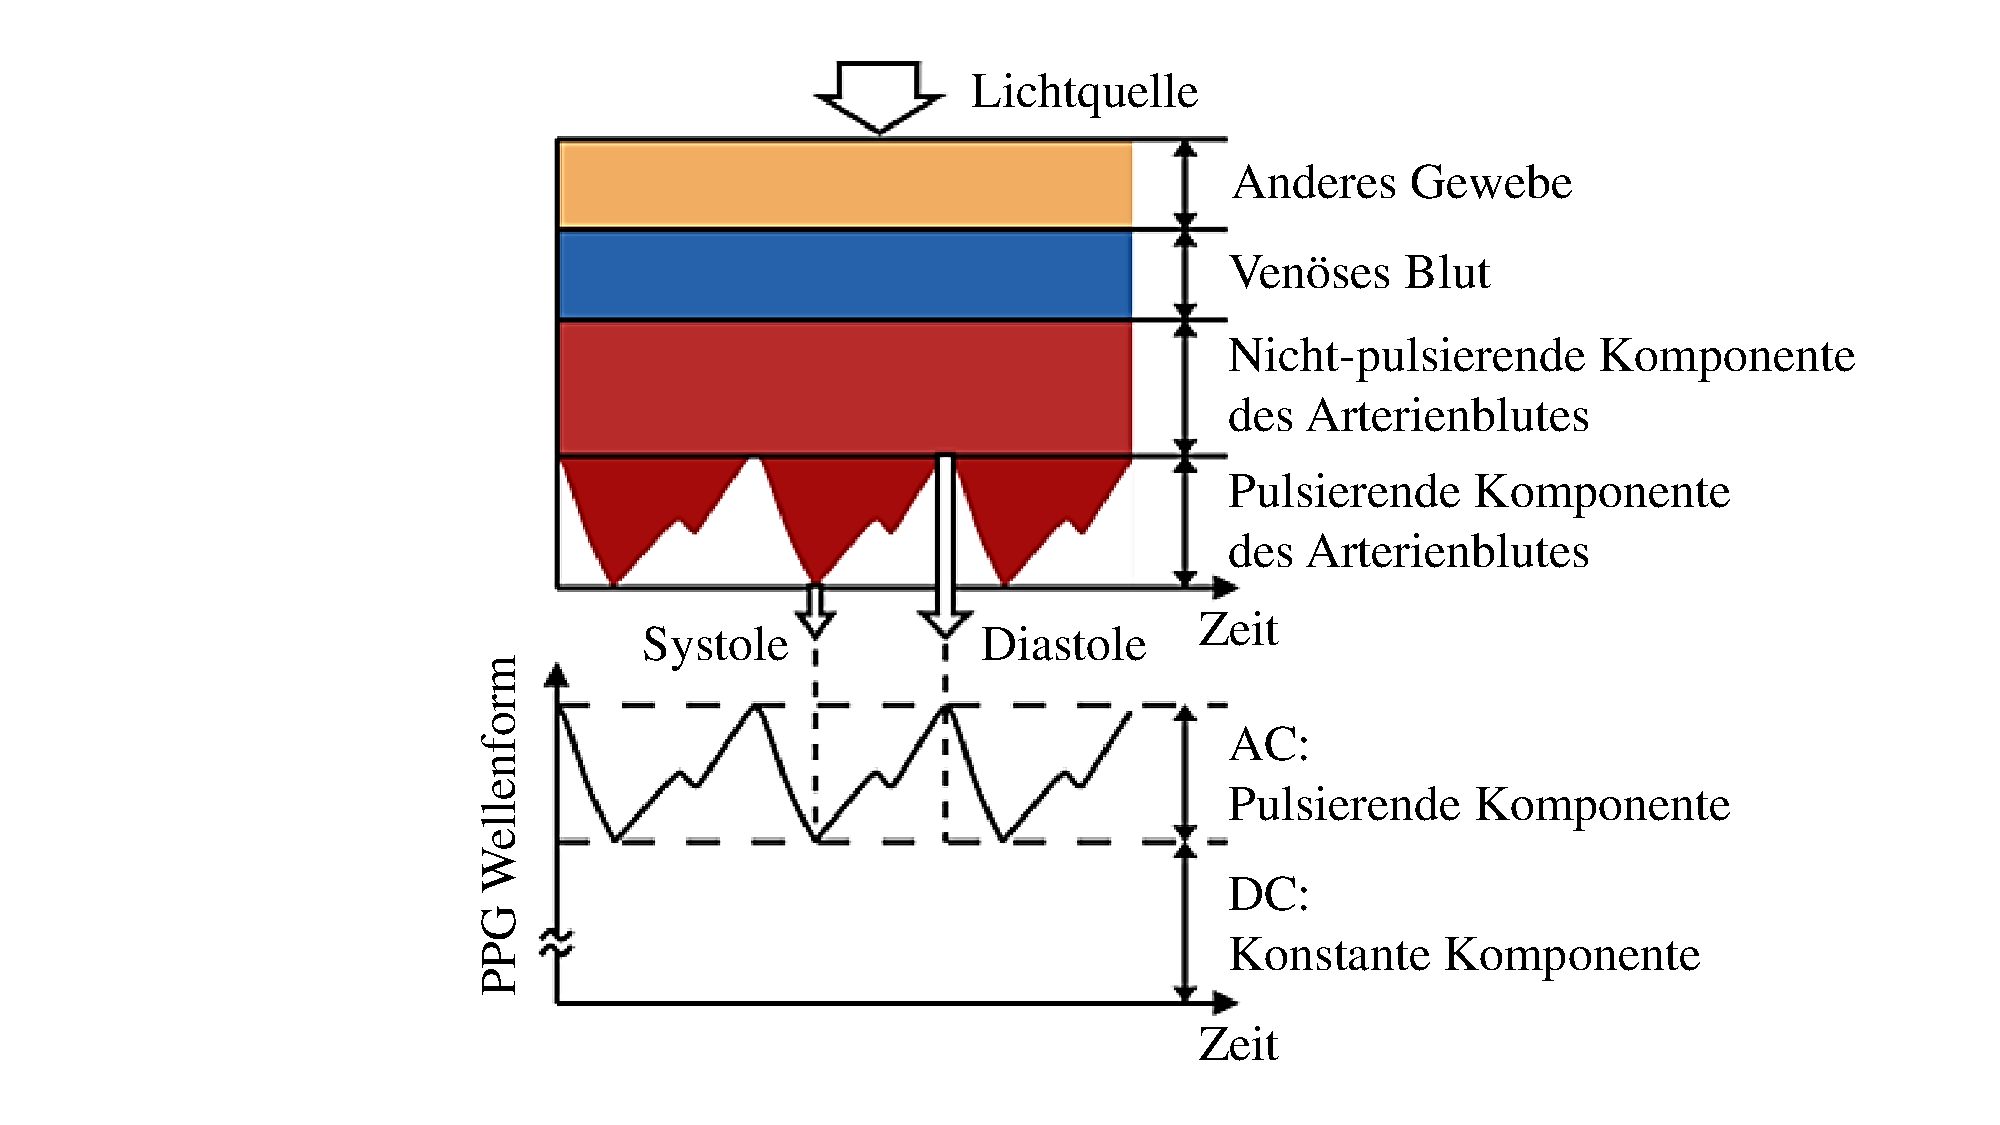
\includegraphics[width=0.9\linewidth]{images/waveform.pdf}
	\caption{Variation der Lichtdämpfung durch Gewebe. Abbildung nach \cite{tamura2014wearable}.}
	\label{waveform}
\end{figure*}

\paragraph{Bioimpedanzanalyse} (BIA) gilt als nicht-invasives, schnelles und zuverlässiges Verfahren um das Gesamtkörperwasser zu bestimmen \cite{kavouras2002assessing}.
Jedoch sind solche Messungen insbesondere außerhalb idealer Laborbedingungen ungenau.
Schweiß, Hauttemperatur, Elektrodenplatzierung und Körperhaltung haben einen Einfluss auf die Messung.
Höchste Genauigkeit wird erst unter standardisierten Bedingungen erreicht, wie z.B. die Reinigung der Haut mit Alkohol vor dem Platzieren der Elektroden, genaue Bestimmung von Körpergröße und Gewicht, das Fasten für 4 Stunden vor der Messung und Vermeidung von sportlicher Aktivität. 
Obwohl BIA als potenzielle Technik zur Beurteilung des Hydratationszustandes vielversprechend ist, sind weitere Untersuchungen erforderlich, bevor es als diagnostisches Instrument zur Untersuchung von Veränderungen des Körperwassers eingesetzt werden kann \cite{garret2018engineering, kavouras2002assessing}.

\section{Tragbare Photoplethysmographie Sensoren}
\label{tragbare photoplethysmographie sensoren}

Neben den etablierten Methoden wurden einige neue Ansätze zur Beurteilung der Hydratation entwickelt.
Darunter findet sich die Verwendung von tragbaren Photopletysmographie Sensoren zur Messung des Hydratationszustandes \cite{kirenko2017unobtrusive, mcpherson2015systems, grudic2017hemodynamic, suryadevara2015towards}.

Um zu beurteilen, ob sich PPG-Sensoren als diagnostisches Instrument eignen, wird im Folgenden zunächst erläutert, wie PPG-Sensoren zur physiologischen Messung genutzt werden können.
Danach werden Möglichkeiten zur Verarbeitung des PPG-Signals aufgezeigt, um daraus den Hydratationszustand einer Person zu bestimmen.

\subsection{Verwendung von Photopletysmographie zur physiologischen Messung}
\label{verwendung von photopletysmographie zur physiologischen messung}

\subsubsection{Prinzip von PPG}
\label{prinzip von ppg}


Das Erfassen einer plethysmographischen Wellenform basiert auf dem Prinzip, dass die Absorption einer bestimmten Wellenlänge der Lichtenergie im Gewebe mit der Menge an sauerstoffhaltigem Blut in Gefäßen wie Arterien oder Arteriolen variiert. 
Wenn das Herz schlägt, nimmt das Blutvolumen zu und wandert als Druckwelle durch den Kreislauf. 
Wenn diese Druckwelle den Sensor passiert, wird mehr Lichtenergie absorbiert, und nachdem die Druckwelle vorbei ist, wird weniger Lichtenergie absorbiert. 
Dieses zeitvariante Signal kann mit einem Sensor erfasst werden, der aus einer Lichtquelle in Kombination mit einem Photodetektor besteht \cite{mcpherson2015systems}.

Der PPG-Sensor überwacht Veränderungen der Lichtintensität durch Reflexion oder Transmission durch das Gewebe.
Das durch das Gewebe wandernde Licht kann von verschiedenen Substanzen absorbiert werden wie den Pigmenten der Haut, den Knochen, arteriellem und venösem Blut.
Die meisten Veränderungen der Durchblutung treten vor allem in den Arterien und Arteriolen auf.
So enthalten Arterien beispielsweise in der systolischen Phase des Herzzyklus mehr Blutvolumen als in der diastolischen Phase.
Blut absorbiert mehr Licht als das umgebende Gewebe.
Daher wird eine Verringerung der Blutmenge als eine Erhöhung der Intensität des erfassten Lichts erkannt \cite{tamura2014wearable}.

Die photoplethysmografische Wellenform enthält Informationen über eine Vielzahl von physiologischen Eigenschaften, einschließlich der relativen Wassermenge im Blut. 
Es wurde festgestellt, dass aus dem Wassergehalt im Blutplasma ein Hinweis auf den Wassergehalt des gesamten Körpers abgeleitet werden kann \cite{mcpherson2015systems}.

Abbildung \ref{waveform} zeigt ein Beispiel für eine photoplethysmografische Wellenform, die aus Gleichstrom- (DC) und Wechselstromkomponenten (AC) besteht.
Die DC-Komponente der PPG-Wellenform entspricht dem detektierten transmittierten oder reflektierten optischen Signal aus dem Gewebe und hängt von der Struktur des Gewebes und dem durchschnittlichen Blutvolumen des arteriellen und venösen Blutes ab.
Die AC-Komponente zeigt Veränderungen des Blutvolumens, die zwischen der systolischen und der diastolischen Phase des Herzzyklus auftreten \cite{tamura2014wearable}.
Die Grundfrequenz der AC-Komponente überlagert die DC-Komponente und ist abhängig von der Herzfrequenz.
Typischerweise liegt die Grundfrequenz der AC-Komponente bei ungefähr 1 Hz \cite{john2007photopletysmography}.
In Abbildung \ref{ekg} sieht man ein PPG-Signal mit dem korrespondierenden Elektrokardiogramm (EKG).

\begin{figure}
	\centering
	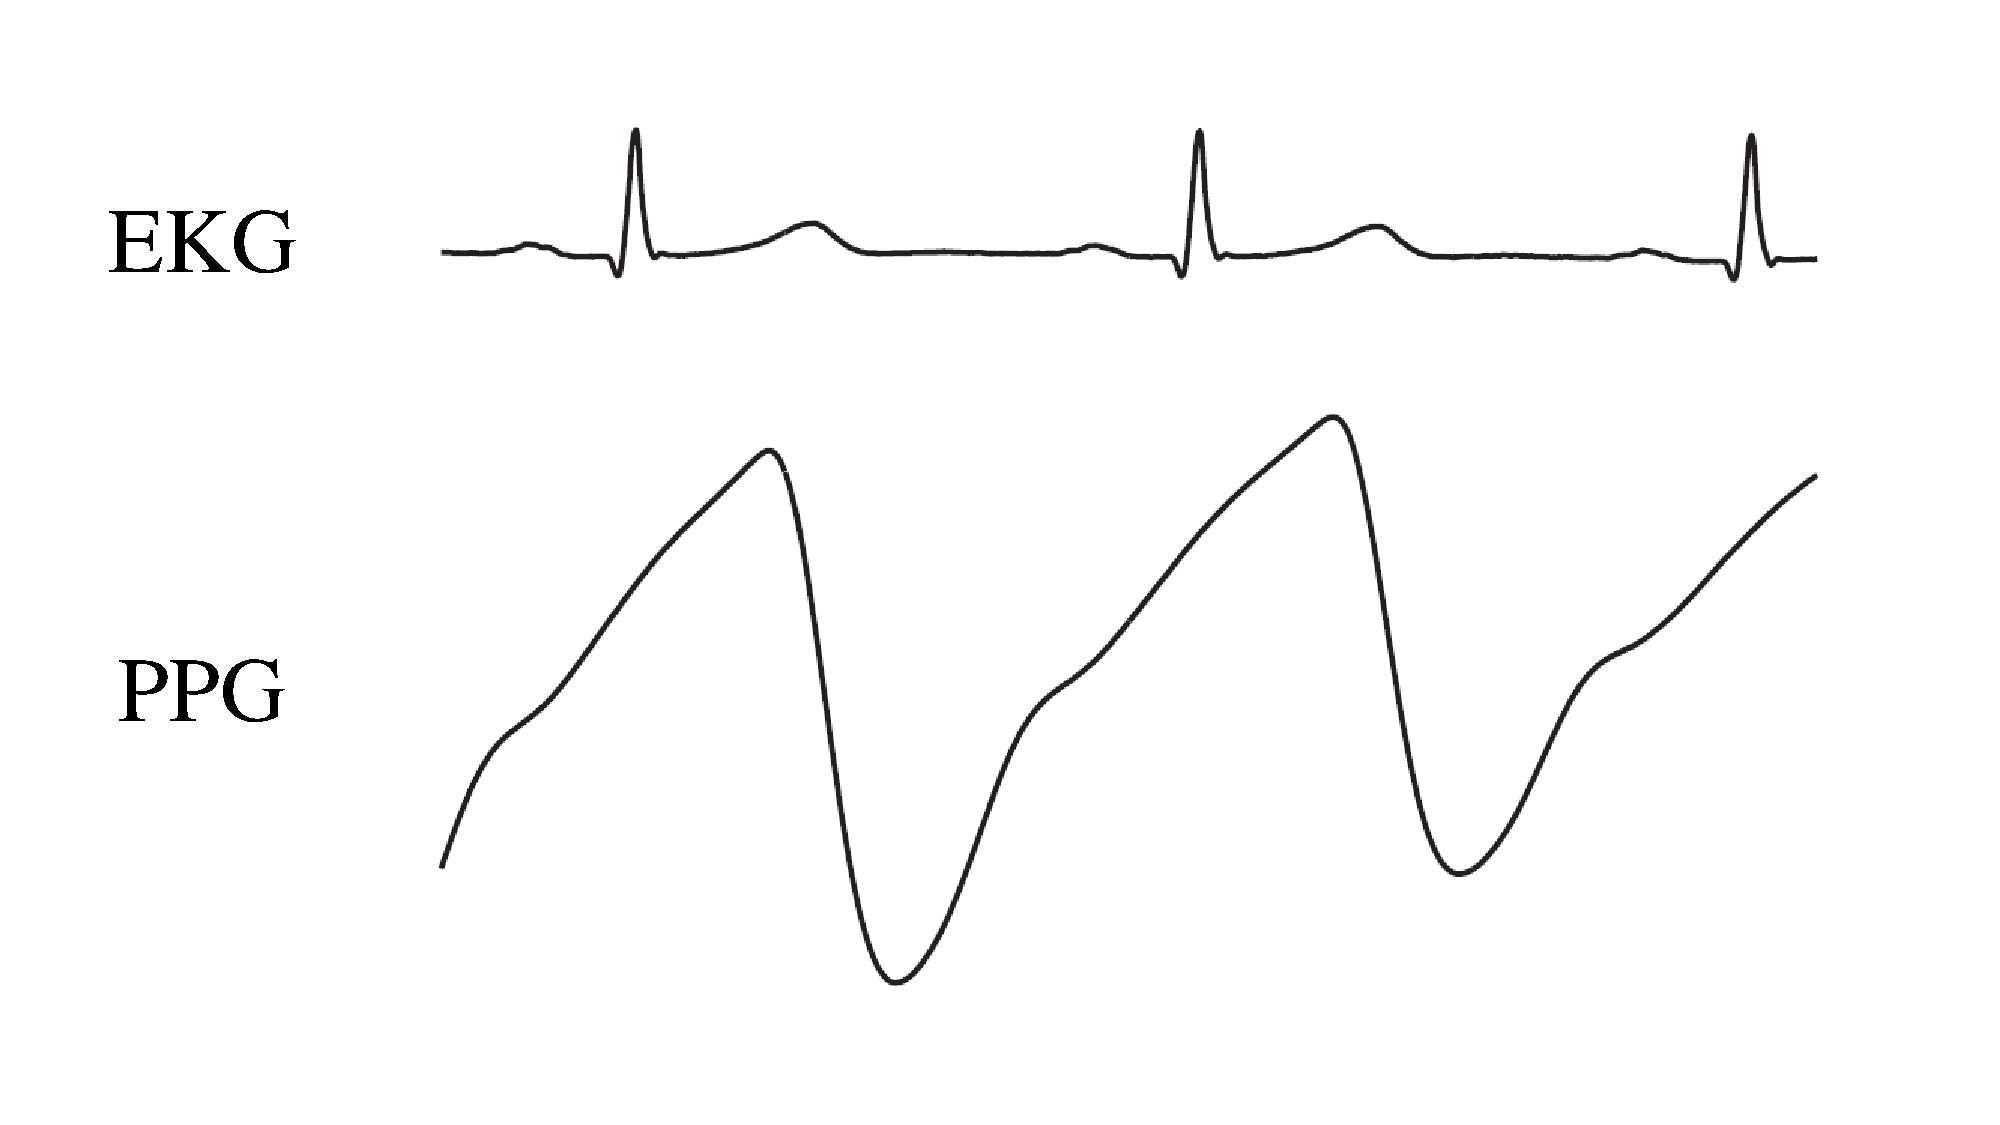
\includegraphics[width=\linewidth]{images/ekgundppg.pdf}
	\caption{Die pulsierende (AC-) Komponente des PPG-Signals und entsprechendes Elektrokardiogramm
(EKG). Sie repräsentiert die erhöhte Lichtdämpfung im Zusammenhang mit der Zunahme des mikrovaskulären Blutvolumens mit jedem Herzschlag. Abbildung nach \cite{john2007photopletysmography}.}
	\label{ekg}
\end{figure}


\begin{figure*}[ht]
	\centering
	\subfloat[][]{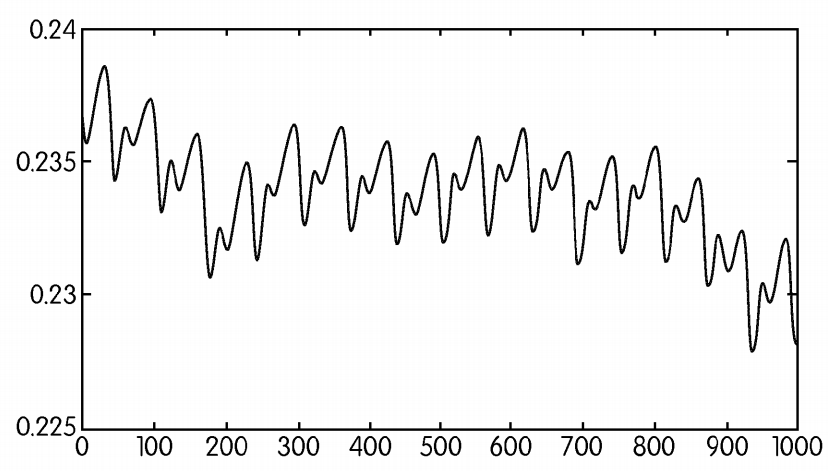
\includegraphics[width=0.6\linewidth]{images/welle_bevor.png}}%
  \qquad
  \subfloat[][]{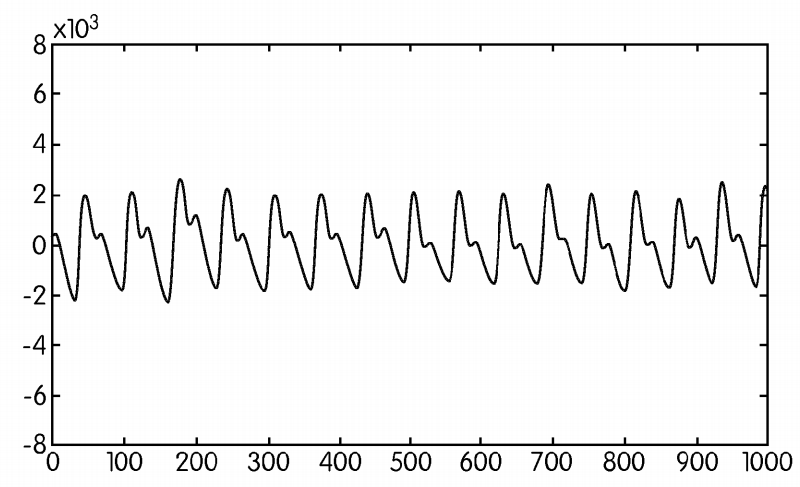
\includegraphics[width=0.6\linewidth]{images/welle_danach.png}}%
	\caption{Bild (a) zeigt eine rohe, uninvertierte plethysmographische Wellenform mit einer geringen Menge an Stromleitungsrauschen und Basislinienwanderung. Bild (b) zeigt das Signal von (a), nachdem es invertiert, gefiltert und die Basislinienwanderung entfernt wurde. Abbildung aus \cite{mcpherson2015systems}.}
	\label{verarbeitung}
\end{figure*}

\subsubsection{Wellenlänge des Lichts}
\label{wellenlaenge des lichts}

Die Wechselwirkung von Licht mit biologischem Gewebe kann sehr komplex sein und kann Streuung, Absorption oder Reflexion beinhalten.
Betrachtet man die Eindringtiefe des Lichts in die menschliche Haut, so entspricht innerhalb des sichtbaren Bereichs der dominante Absorptionspeak dem blauen Bereich des Spektrums.
Dem folgt der grün-gelbe Bereich (zwischen 500 und 600nm), der von den roten Blutkörperchen absorbiert wird.
Die kürzeren Wellenlängen des Lichts werden stark von Melanin absorbiert.
Wasser absorbiert Licht im ultravioletten und längeren infraroten Bereich, wobei rotes und nahezu infrarotes Licht leicht passieren kann \cite{anderson1981optics}.

Die Wellenlänge und der Abstand zwischen Lichtquelle und Photodetektor (PD) bestimmen die Eindringtiefe des Lichts. 
Grünes Licht eignet sich zur Messung der oberflächlichen Durchblutung der Haut.
Infrarote oder nahinfrarote Wellenlängen eignen sich besser für die Messung des tiefen Gewebedurchflusses (z.B. Durchblutung der Muskeln). 

Daraus folgend werden rote und infrarote Wellenlängen oft als Lichtquelle in PPG-Sensoren verwendet.
Allerdings werden PPG-Geräte mit grüner Wellenlänge  immer beliebter, da eine grüne lichtemittierende Diode (LED) eine wesentlich höhere Absorptionsfähigkeit sowohl für Oxyhämoglobin als auch für Desoxyhämoglobin im Vergleich zu Infrarotlicht hat.
Daher ist die Veränderung des reflektierten grünen Lichts größer als die des reflektierten infraroten Lichts, wenn Blut durch die Haut fließt, was zu einem besseren Signal-Rausch-Verhältnis für die grüne Lichtquelle führt \cite{john2007photopletysmography}.


\begin{figure*}[ht]
	\centering
	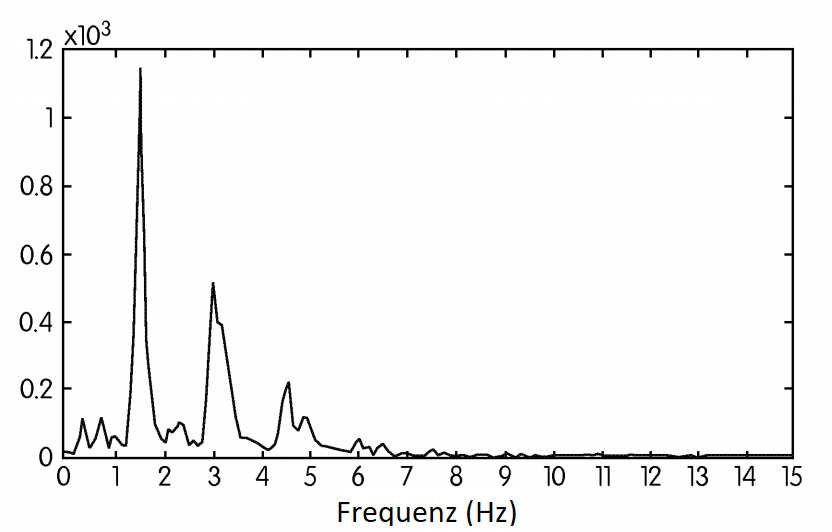
\includegraphics[width=0.6\linewidth]{images/welle_fft.png}
	\caption{Frequenzspektrum der plethysmographischen Wellenform aus Abbildung \ref{verarbeitung}, das mit einem Fast Fourier Transform Algorithmus abgeleitet wurde. Abbildung nach \cite{mcpherson2015systems}.}
	\label{fft}
\end{figure*}

\subsubsection{Transmittierte und reflektierte Signale}
\label{transmittierte und reflektierte signale}

\begin{figure*}[ht]
	\centering
	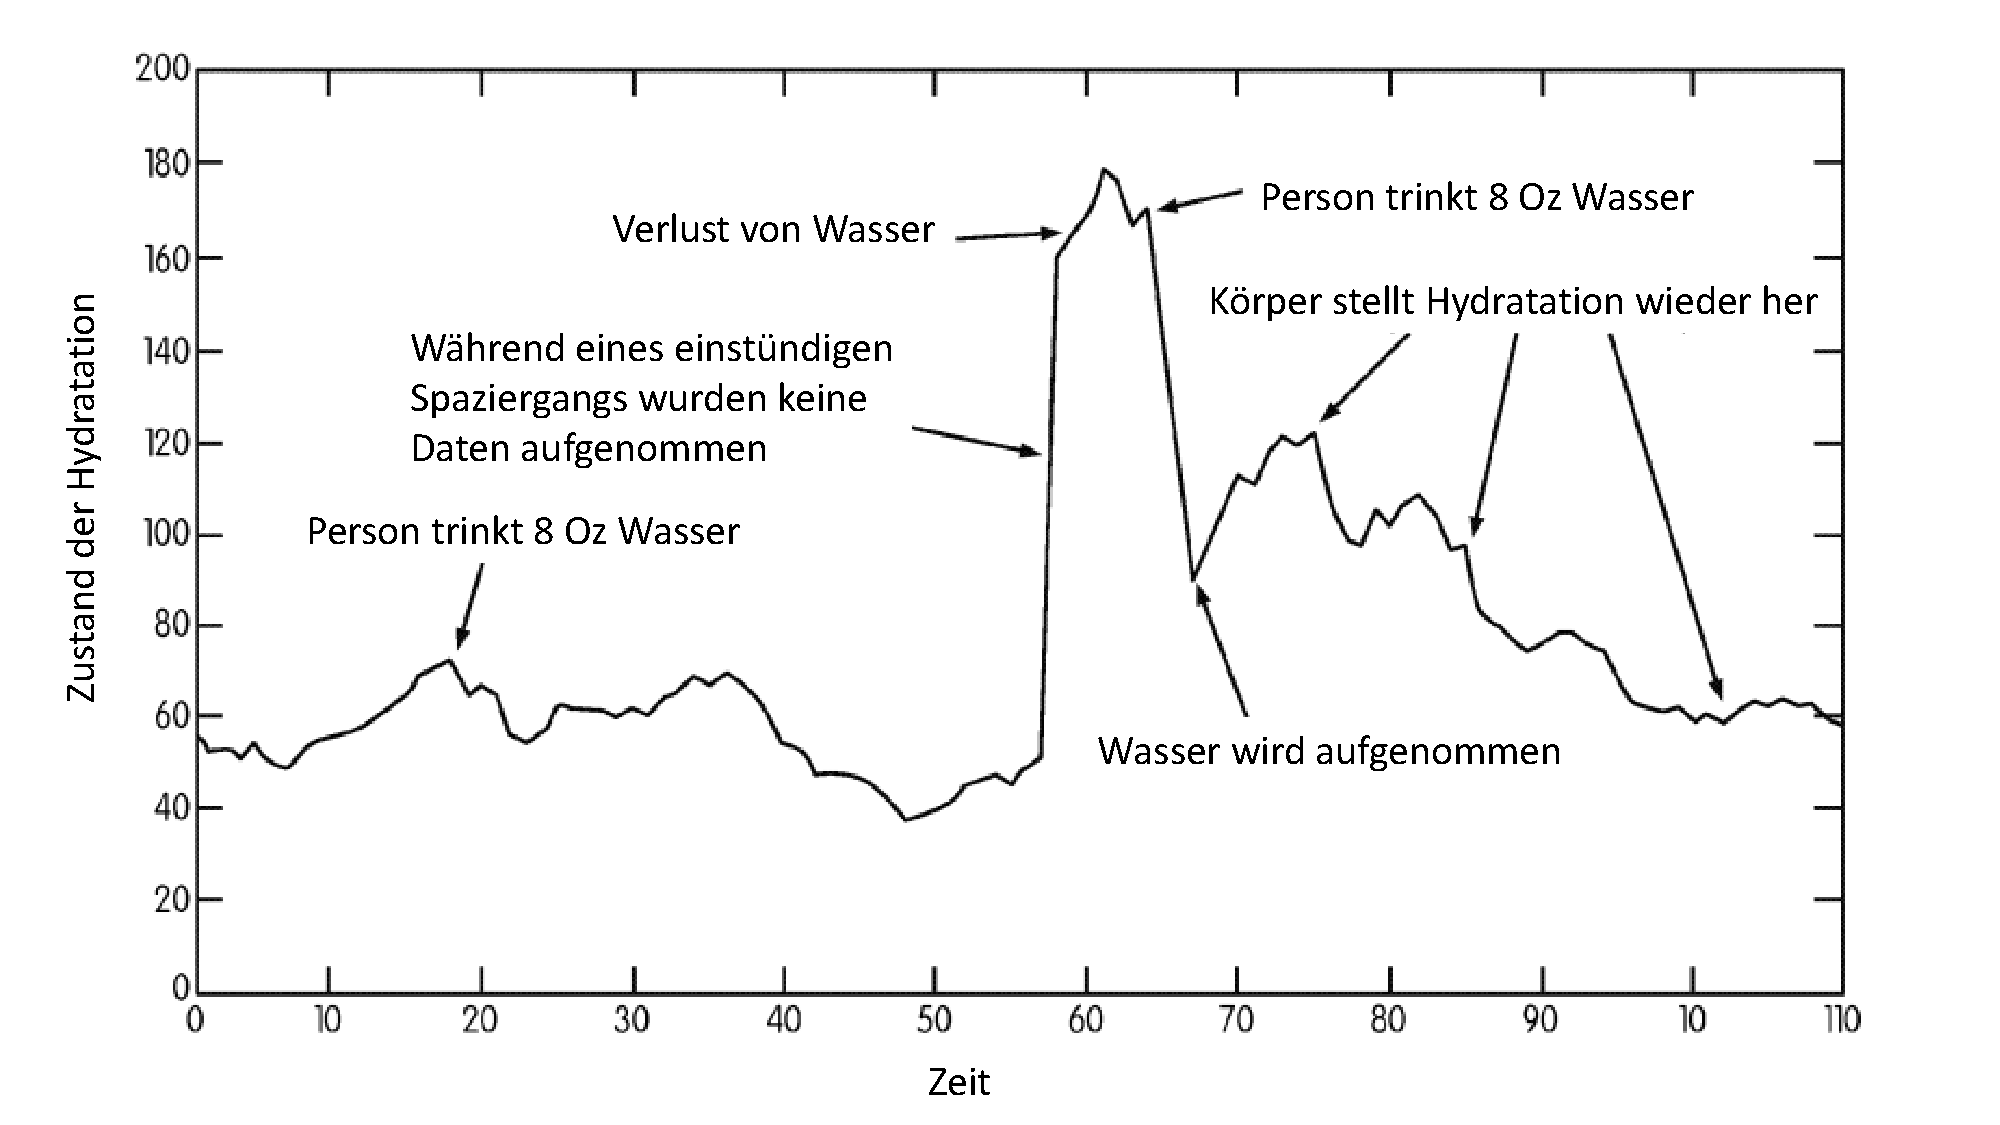
\includegraphics[width=\linewidth]{images/hydratationsdaten.pdf}
	\caption{Beispiel für reale Hydratationsdaten, die über das Verfahren von \textbf{McPherson et al.} gesammelt wurden, wobei die X-Achse die Zeit und die y-Achse den Hydratationszustand als Funktion der Größe der primären Harmonischen anzeigt. Abbildung nach \cite{mcpherson2015systems}.}
	\label{hydratationszustand}
\end{figure*}

Bei der Messung des PPG-Signals gibt es zwei Modi.
Beim Transmissionsmodus befindet sich die Gewebeprobe (z.B. Fingerkuppe) zwischen der Lichtquelle und dem Detektor.
Im Reflexionsmodus befinden sich Lichtquelle und Detektor nebeneinander, wobei der Detektor das Licht einfängt, welches vom Gewebe zurückgestrahlt wird \cite{john2007photopletysmography}.

Im Transmissionsmodus kann ein relativ gutes Signal erhalten werden, aber die Messstellen sind begrenzt.
Der Sensor muss am Körper an einer Stelle platziert werden, die durchleuchtet werden kann, wie z.B. Fingerspitze, Nasenscheidewand, Wange, Zunge und Ohrläppchen.
Fingerspitze und Ohrläppchen sind die bevorzugten Überwachungspositionen, jedoch haben diese Stellen eine begrenzte Durchblutung.
Darüber hinaus sind die Fingerspitze und das Ohrläppchen anfälliger für Umweltextreme, wie z.B. niedrige Umgebungstemperaturen.
Der größte Nachteil an der Platzierung an der Fingerspitze ist, dass der Sensor im Alltag als störend empfunden werden könnte \cite{tamura2014wearable}.

Der Reflexionsmodus beseitigt die mit der Sensorplatzierung verbundenen Probleme und es können verschiedene Messstellen verwendet werden.
Der Reflexionsmodus des PPG wird jedoch durch Bewegungsartefakte und Druckstörungen beeinflusst.
Jede Bewegung, wie z.B. körperliche Aktivität, kann zu Bewegungsartefakten führen, die das PPG-Signal stören und die Messgenauigkeit physiologischer Parameter einschränken.
Auf die Sonde einwirkende Druckstörungen, wie z.B. die Kontaktkraft zwischen PPG-Sensor und Messstelle, können die arterielle Geometrie durch Kompression verformen.
So kann im reflektierten PPG-Signal die AC-Amplitude durch den auf die Haut ausgeübten Druck beeinflusst werden \cite{tamura2014wearable}.

\subsection{Verarbeitung des PPG-Signals}
\label{verarbeitung des ppg-signals}

Um aus dem reinen PPG-Signal den Hydratationsstatus einer Person bestimmen zu können, muss dieses zunächst verarbeitet werden.
\textbf{McPherson et al.} haben eine Messanordnung entwickelt und patentiert, die durch algorithmische Merkmalsextraktion aus einer plethysmographischen Wellenform den Hydratationsstatus bestimmen kann. 
Das System verwendet eine einzige monochromatische Lichtquelle, zum Beispiel eine LED, mit den Wellenlängen von 400 nm bis 2000 nm und einen Photodetektor, wie zum Beispiel eine PIN-Fotodiode.
Zudem wird ein Bewegungssensor verwendet, wie beispielsweise ein Beschleunigungssensor oder Gyroskop, der die Relativbewegung der Sensorumgebung misst, die dazu neigt, die plethysmografische Wellenform zu verzerren. 
Diese Bewegungsinformationen können anschließend von der verzerrten plethysmografischen Wellenform subtrahiert werden, wodurch die Wiederherstellung der wahren plethysmografischen Wellenform von der verzerrten Wellenform ermöglicht wird \cite{mcpherson2015systems}.

Eine ähnliche Messanordnung wird auch von \textbf{Kirenko et al.} genutzt.
Dabei werden mehrere PPG-Signale genutzt, um eine Fernüberwachung des Hydratationszustandes von Hautgewebe zu ermöglichen.
Die Vorrichtung umfasst eine Schnittstelle zum Empfangen eines Datenstroms, der eine Vielzahl von PPG-Signalen umfasst, eine Verarbeitungseinheit und
einer Analyseeinheit zum Berechnen eines Hydratationssignals, das die Hautfeuchtigkeit anzeigt \cite{kirenko2017unobtrusive}.

\textbf{Suryadevara et al.} entwickelten ein tragbares Messgerät, welches einen PPG-Sensor mit der Messung der Hauttemperatur und der elktrodermalen Aktivität kombiniert.
Diese drei Parameter werden zusammen mit dem Body-Mass-Index des Benutzers in eine empirisch abgeleitete Formel eingegeben und die Schätzung für die Menge der verlorenen Flüssigkeit wird bestimmt. \cite{suryadevara2015towards}.

Bevor die plethysmographische Wellenform analysiert werden kann, müssen die Rohdaten verarbeitet werden, um Rauschen und Basislinienwanderungen zu vermeiden. 
Die Daten können auch invertiert werden, um die Wellenform dem üblichen plethysmographischen Standard anzupassen, aber dies dient der Übersichtlichkeit und ist keine absolute Voraussetzung für die Verarbeitung der Daten. 
Die plethysmographische Wellenform kann in umgekehrter oder nicht umgekehrter Form verarbeitet werden \cite{mcpherson2015systems}.

Rauschen in der Wellenform kann entweder durch elektrische oder mechanische Faktoren verursacht werden, wie z.B. 60 Hz Netzrauschen oder eine mechanische Vibration, die in den Patienten induziert wird. 
Basislinienwanderung ist die sich langsam ändernde DC-Vorspannungsvariation, die durch geringfügige Änderungen der DC-Vorspannung der Sensorverstärker verursacht wird, was zu einem DC-Versatz in der Wellenform führt. 
Abbildung \ref{verarbeitung} (a) zeigt eine rohe, uninvertierte plethysmographische Wellenform mit einer geringen Menge an Stromleitungsrauschen und Basislinienwanderung \cite{mcpherson2015systems}.

Die richtige Wahl der Abtastfrequenz und eine Tiefpassfilterung des Signals reichen in der Regel aus, um das elektrische Rauschen aus dem Signal zu entfernen \cite{mcpherson2015systems, suryadevara2015towards}. 
Die Basislinienwanderung wird durch Subtraktion des Langzeitmittelwerts des Signals entfernt. 
Abbildung \ref{verarbeitung} (b) zeigt das Signal von Abbildung \ref{verarbeitung} (a), nachdem es invertiert, gefiltert und die Basislinienwanderung entfernt wurde. 
Die plethysmographische Wellenform in Abbildung \ref{verarbeitung} (b) ist ein Beispiel für eine plethysmographische Wellenform, die durch die Messung der Absorption von Infrarotlicht, das durch sauerstoffreiches Gewebe übertragen wird, erhalten wird.
Die Spitze der Wellenform entspricht der maximalen Absorption des IR-Lichts, wenn die Blutgefäße, wie z.B. Arteriolen, bei ihrer maximalen Ausdehnung pulsieren, und der niedrigste Teil der Wellenform ist der Punkt zwischen den Herzschlägen, an dem es die minimale Ausdehnung der Gefäße und entsprechend weniger Absorption des Lichts gibt \cite{mcpherson2015systems}.

Sobald das Signal so verarbeitet wurde, dass es symmetrisch um Null herum periodisch ist, wobei alle DC-Vorspannungen entfernt wurden, ist die Wellenform bereit für die Merkmalsextraktion, um die Menge an Wasser im Blut zu bestimmen.
Der Hydratationsstatus der Person basiert auf der Größe der Spitzenfrequenz.
Im Allgemeinen gilt: Je kleiner die Spitzenfrequenz, desto wahrscheinlicher ist es, dass die Person Wasser verliert. 
Die genaue Größe zur Unterscheidung zwischen einem ausreichend hydratisierten Zustand und einem Zustand der Dehydrierung variiert von Person zu Person. 
Daher muss das System individuell kalibriert werden \cite{mcpherson2015systems}. 


Eine Möglichkeit der Merkmalsextraktion ist ein Frequenzspektrum der Wellenform durch den Einsatz der Fourier-Transformationsanalyse zu erhalten.
Eine Fourier-Transformation wandelt Zeit- oder Rauminformationen in Frequenzen um. 
Von besonderem Nutzen ist das als Fast Fourier Transform (FFT) bekannte Verfahren, mit dem ein diskreter Datensatz rechnerisch schnell und effizient verarbeitet werden kann. 
Algorithmisch ist die Größe der Maxima des Frequenzspektrums, die von einer Fourier-Transformation zurückgegeben werden, insbesondere der ersten (primären) Harmonischen einer plethysmographischen Wellenform, umgekehrt proportional zum Hydratationsstatus des Individuums, von dem die Wellenform genommen wird. 
Abbildung \ref{fft} zeigt ein Beispiel für eine FFT, die aus dem Plethysmographen von Abbildung \ref{verarbeitung} erhalten wurde. 
Die erste Harmonische kann als der große Anstieg in der Wellenform beobachtet werden.
Die Größe der FFT-Primärharmonischen korreliert mit der Menge des Blutvolumens, von dem Wasser die größte Komponente ist \cite{mcpherson2015systems}.


Abbildung \ref{hydratationszustand} zeigt ein Beispiel für reale Hydratationsdaten, die über das Verfahren von \textbf{McPherson et al.} gesammelt wurden, wobei die X-Achse die Zeit und die y-Achse den Hydratationszustand als Funktion der Größe der primären Harmonischen anzeigt.



\section{Schlussbetrachtung und Ausblick}
\label{schlussbetrachtung und ausblick}

In Kapitel \ref{tragbare photoplethysmographie sensoren} wurde erklärt, wie Photopletysmographie Sensoren zur Bestimmung des Hydratationszustandes einer Person genutzt werden können.
Sie umgehen sogar einige Probleme, die bei den etablierten klinischen Diagnosen und Laboruntersuchungen auftreten.

Eine klinische Anamnese ist im Allgemeinen nicht ausreichend sensitiv und spezifisch. 
Zudem sind Faktoren wie Durst sehr subjektiv und ungenau.
Im Vergleich dazu sind Messungen mit PPG-Sensoren sehr objektiv und können nach einer Kalibrierung der Algorithmen auf die Versuchsperson genauere Ergebnisse liefern.

Urinanalysen lassen keine kontinuierliche Überwachung zu.
Sie sind ungenau, erfordern technische Kompetenz und erbringen verzögerte Ergebnisse.
Blutanalysen sind weniger empfindlich als Urinanalysen, sind kostspielig und benötigen viel Zeit.
Zudem erfordern sie wie im Fall des klinischen Standards der Plasma-Osmolalität eine Venenpunktion, was sie invasiv macht.
Messungen des Gewichts sind nur über kurze Zeiträume genau.
Die Bioimpedanzanalyse erfordert ideale Laborbedingungen und ist außerhalb dieser ungenau.

PPG-Sensoren sind nicht invasiv, sie sind relativ günstig, tragbar und können kontinuierlich Veränderungen des Körperwassers messen.
Sie erfordern technische Kompetenz nur beim Entwickler der Messanordnung oder des tragbaren Gerätes, das die PPG-Signale auswertet. 
Sie eignen sich besonders um den Hydratationszustand über längere Zeiträume zu überwachen. 

Die Genauigkeit und Relevanz der Auswertung der PPG-Signale hängt von der Qualität der verwendeten Algorithmen bei der Verarbeitung und Merkmalsextraktion ab.
In Zukunft können diese Algorithmen noch weiter verfeinert werden und zu genaueren und verlässlicheren Ergebnissen führen.
So könnten die tragbaren Geräte im Alltag vieler von Dehydratation gefährdeter Personengruppen eingesetzt werden.



%
%%%%%%%%%%%%%%%%%%%%%%%%%%%%%%%%%%%%%%%%%%%%%%%%%%%%%%%%%%%%%%%%%%%%%%%%%%%%%%%%%%%%
% Literaturverzeichnis
\printbibliography
% Anhang
%\appendix
%\section{Anhang}
%\label{anhang}
\end{document}

